\documentclass[border=0.125cm]{standalone}
\usepackage[swedish]{babel}	
\usepackage[utf8]{inputenc}	
\usepackage{tikz}
\usetikzlibrary{backgrounds,calc,positioning}
\usetikzlibrary{arrows}



\begin{document}


\definecolor{klight_green_400}{RGB}{156, 204, 101}

\tikzset{%
  project part/.style={
    rectangle,
    draw,
    fill=klight_green_400,
    thick,
    minimum width=3.2cm,
    minimum height=1.2cm
  },
  main line/.style={
    draw,
    line width=0.25mm,
    opacity=1,
    minimum size=1cm
  },
}

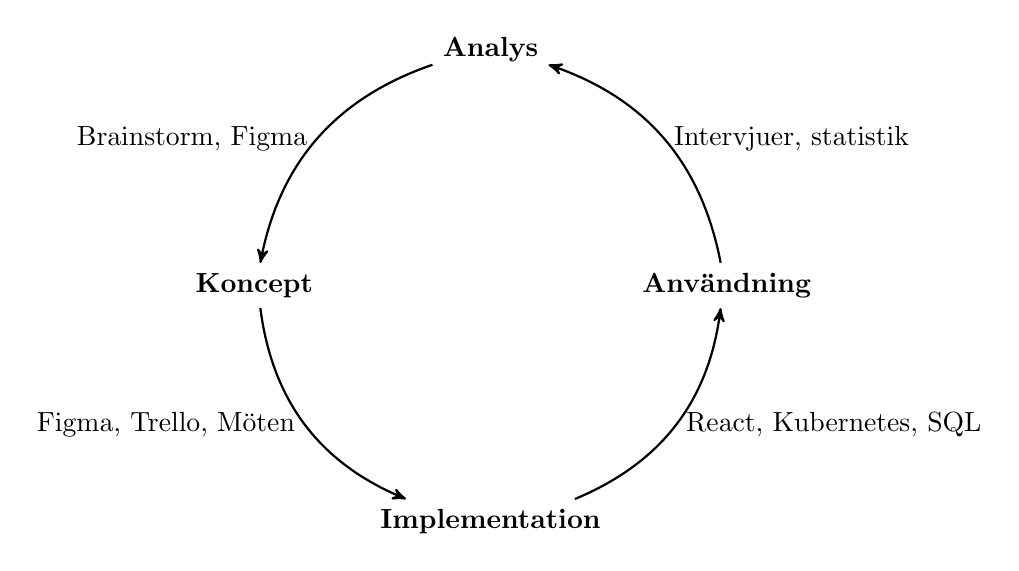
\begin{tikzpicture}[x=1.5cm, y=1.5cm, ->,>=stealth',auto, thick]
% Base project nodes
\node [project part/.try] (collect) at (2,2) {$\textbf{Analys}$};
\node [project part/.try] (concept) at (0,0) {$\textbf{Koncept}$};
\node [project part/.try] (use) at (4,0) {$\textbf{Användning}$};
\node [project part/.try] (implement) at (2,-2) {$\textbf{Implementation}$};


% Connect them 
\path[main line/.style={font=\sffamily\small}]
    (collect) edge[bend right] node [left] {Brainstorm, Figma} (concept)
    (concept) edge[bend right] node [left] {Figma, Trello, Möten} (implement)
    (implement) edge[bend right] node [right] {React, Kubernetes, SQL} (use)
    (use) edge[bend right] node [right] {Intervjuer, statistik} (collect);
\end{tikzpicture}

\end{document}